\documentclass[border=10pt]{standalone}

\usepackage{tikz}
\usepackage{tikzsymbols}
\usetikzlibrary{calc,patterns,shapes.geometric}

\def\centerarc[#1](#2)(#3:#4:#5){\draw[#1] ($(#2)+({#5*cos(#3)},{#5*sin(#3)})$) arc (#3:#4:#5);}

\begin{document}
	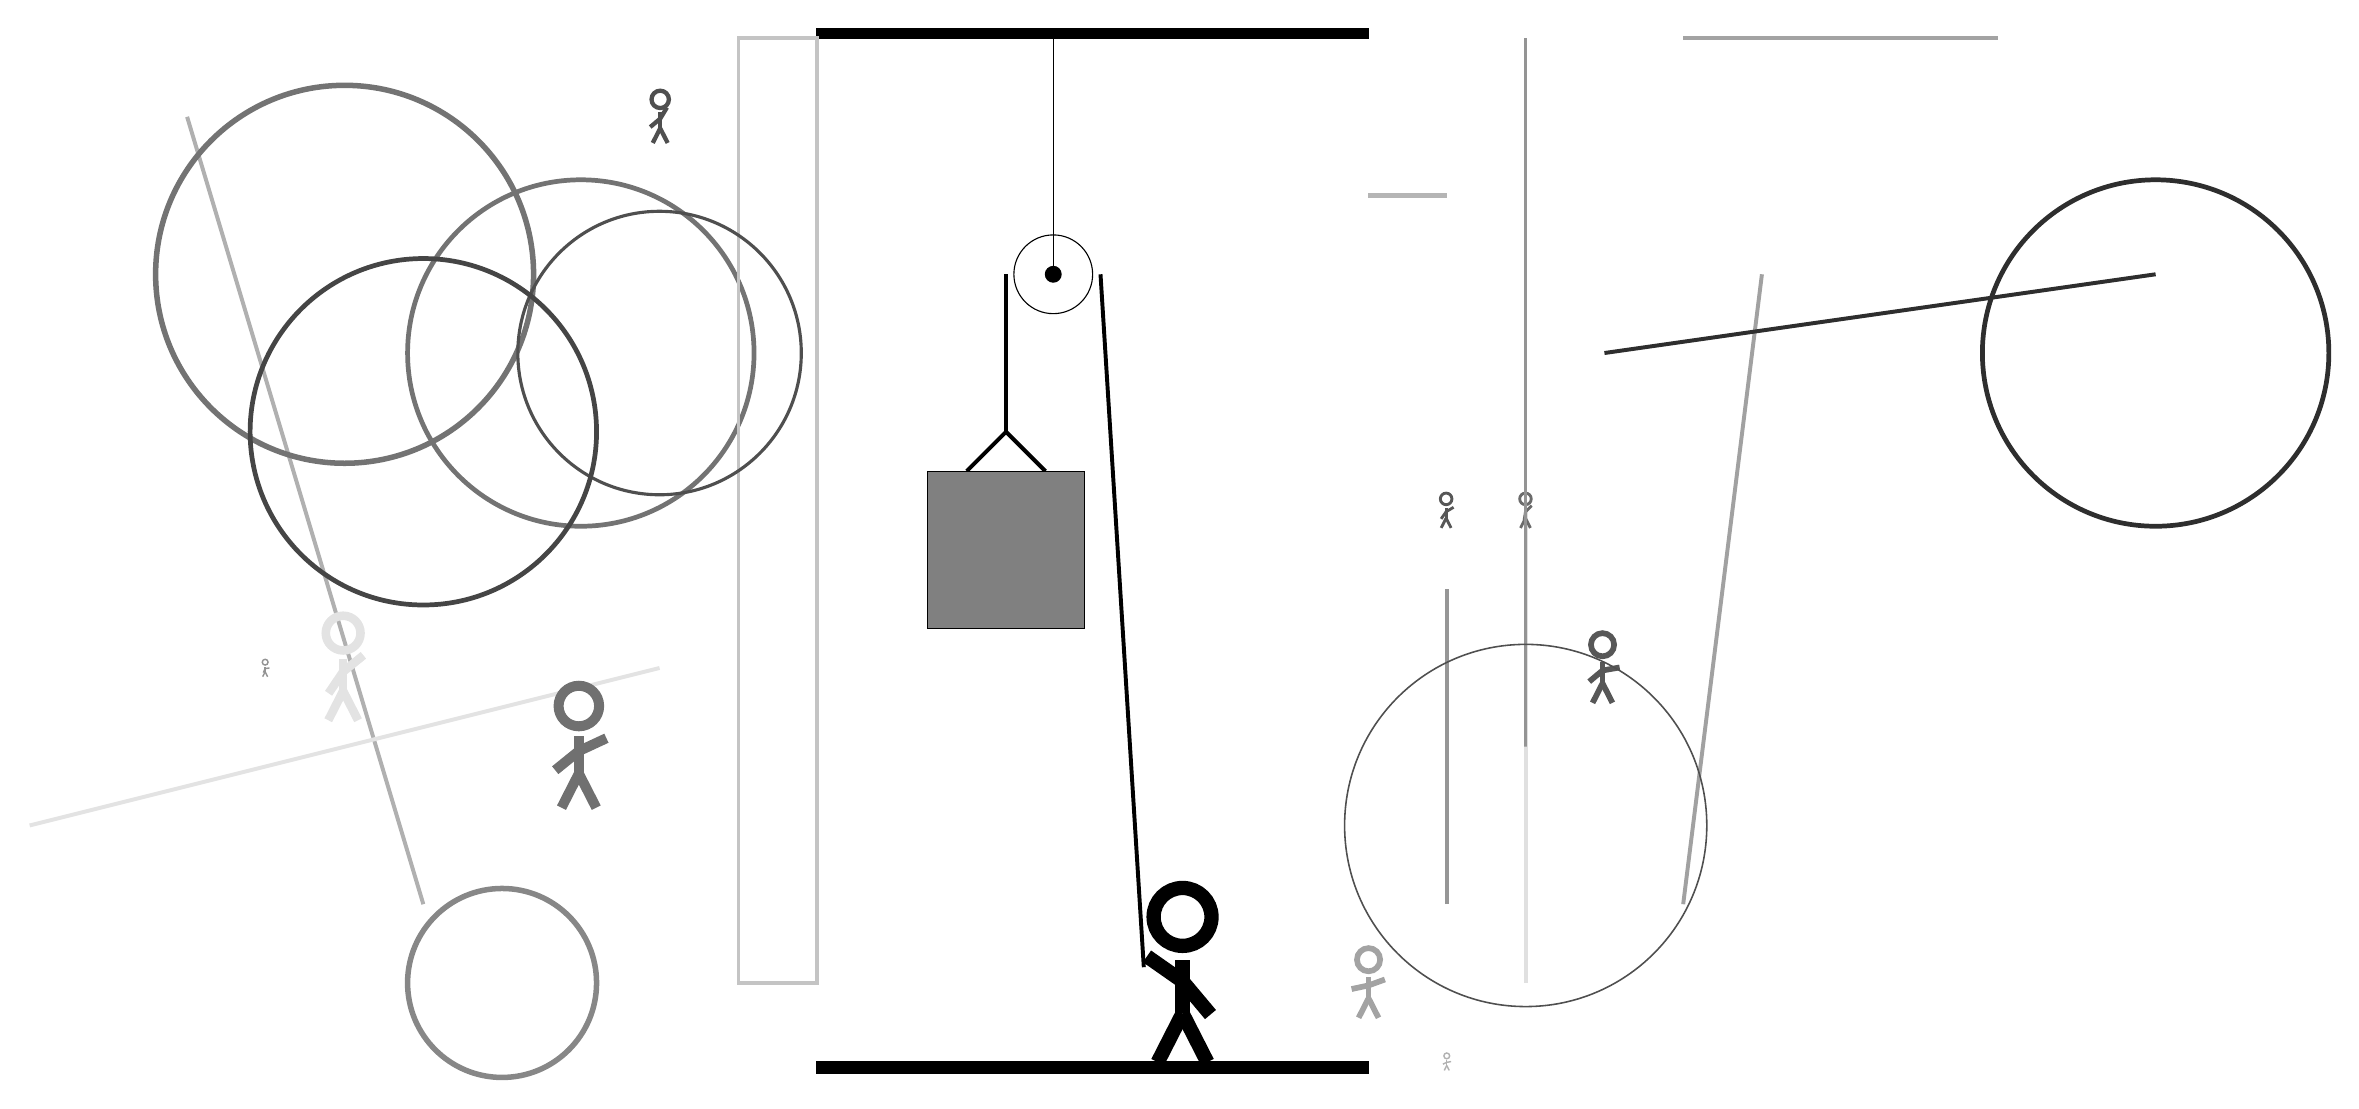
\begin{tikzpicture}
		%%%%% START %%%%%
		
		\draw[fill=black] (-2, 10) rectangle (5, 10.125);
		
		\draw [line width=0.6mm, color=black!55](-5, 6) circle (2.2);
		
		\draw[line width=0.5mm, color=black!31](-7, -1) -- (-10, 9);
		\node[line width=0.5mm, color=black!42] at (-9, 2) {\Strichmaxerl[1][65][9]};
		\node[line width=0.3mm, color=black!30] at (6, -3) {\Strichmaxerl[1][26][9]};
		\draw[line width=0.4mm, color=black!23] (-3, 10) rectangle (-2, -2);
		\draw [line width=0.6mm, color=black!82](15, 6) circle (2.2);
		\draw [line width=0.7mm, color=black!55](-8, 7) circle (2.4);
		\draw [line width=0.4mm, color=black!69](-4, 6) circle (1.8);
		\draw[line width=0.6mm, color=black!29] (5, 8) rectangle (6, 8);
		\draw[line width=0.5mm, color=black!37](9, -1) -- (10, 7);
		\draw[line width=0.5mm, color=black!11](-4, 2) -- (-12, 0);
		\node[line width=0.6mm, color=black!56] at (-5, 1) {\Strichmaxerl[7][39][25]};
		\node[line width=0.2mm, color=black!69] at (-4, 9) {\Strichmaxerl[3][40][59]};
		
		\node[line width=0.7mm, color=black!11] at (-8, 2) {\Strichmaxerl[6][56][39]};
		\draw[line width=0.5mm, color=black!12](7, -2) -- (7, 4);
		\draw[line width=0.5mm, color=black!36](9, 10) -- (13, 10);
		\draw [line width=0.6mm, color=black!73](-7, 5) circle (2.2);
		\draw[line width=0.5mm, color=black!82](8, 6) -- (15, 7);
		\node[line width=0.7mm, color=black!66] at (8, 2) {\Strichmaxerl[4][40][10]};
		\draw[line width=0.5mm, color=black!41](6, -1) -- (6, 3);
		\node[line width=0.6mm, color=black!58] at (7, 4) {\Strichmaxerl[2][81][44]};
		\node[line width=0.7mm, color=black!36] at (5, -2) {\Strichmaxerl[4][12][20]};
		
		\node[line width=0.2mm, color=black!66] at (6, 4) {\Strichmaxerl[2][55][31]};
		\draw[line width=0.4mm, color=black!42] (7, 1) rectangle (7, 10);
		\draw [line width=0.2mm, color=black!69](7, 0) circle (2.3);
		
		\draw [line width=0.7mm, color=black!47](-6, -2) circle (1.2);
		
		\draw (1, 7) circle (0.5);
		\draw[fill=black] (1, 7) circle (0.1);
		\draw (1, 10) -- (1, 7);
		
		\draw[line width=0.5mm] (-0.1, 4.5) -- (0.4, 5.0) -- (0.9, 4.5);
		\draw[fill=black!50] (-0.6, 4.5) rectangle (1.4, 2.5);
		
		\draw[line width=0.5mm] (0.4, 7) -- (0.4, 5.0);
		\centerarc[line width=0.5mm](1, 7)(0:180:0.6);
		\draw[line width=0.5mm](1.6, 7) -- (2.15, -1.8);
		
		\node at (2.6, -1.9) {\Strichmaxerl[10][-35][-50]};
		
		\draw[fill=black] (-2, -3) rectangle (5, -3.15);
		
		%%%%% END %%%%%
	\end{tikzpicture}
\end{document}